\chapter{Deep Learning for Anomaly Detection: A Survey}
% \chapter{Introduction}
\label{chpt:survey}
\section{Introduction}

A common need when analysing real-world datasets is determining which instances stand out as being dissimilar to all others. Such instances are known as \emph{anomalies}, and the goal of \emph{anomaly detection} (also known as \emph{outlier detection}) is to determine all such instances in a data-driven fashion~\cite{chandola2007outlier}. Anomalies can be caused by errors in the data but sometimes are indicative of a new, previously unknown, underlying process; in fact Hawkins~\cite{hawkins} defines an outlier as an observation that {\it deviates so significantly from other observations as to arouse suspicion that it was generated by a different mechanism.} In the broader field of machine learning, the recent years have witnessed proliferation of deep neural networks, with unprecedented results across various application domains. Deep learning is subset of machine learning that achieves good performance and flexibility by learning to represent the data as nested hierarchy of concepts within layers of neural network. Deep learning outperforms the traditional machine learning as the scale of data increases as illustrated in Figure~\ref{fig:performanceCompare}. In recent years, deep learning-based anomaly detection algorithms has become increasingly popular and has been applied for diverse set of tasks as illustrated in Figure~\ref{fig:applications}; studies have shown that deep learning completely surpasses traditional methods~\cite{javaid2016deep,peng2015multi}  in both research and applications ~\cite{javaid2016deep}.

%performance comparision
\begin{figure}[h]
\centering
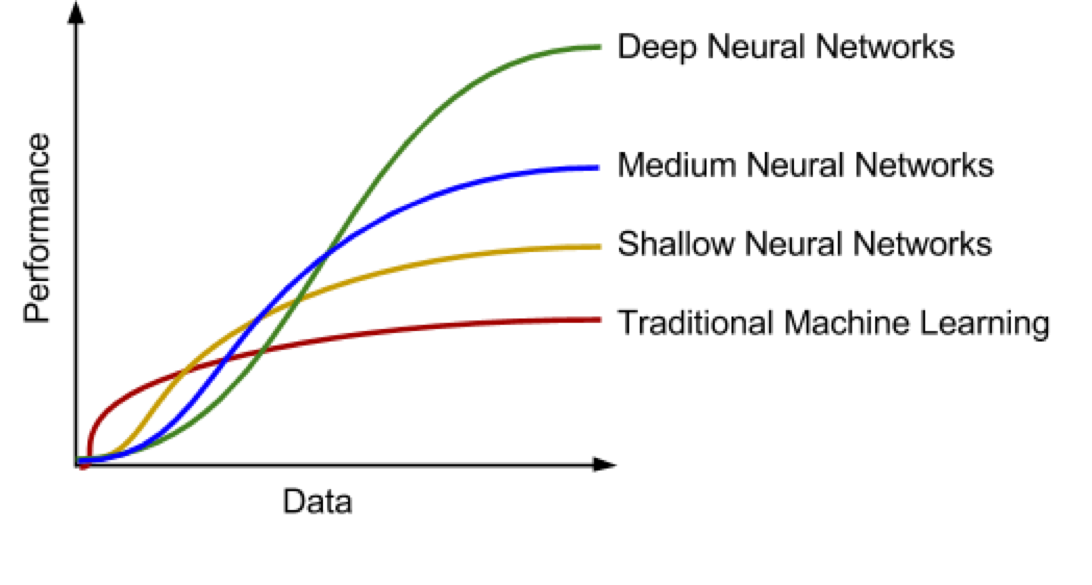
\includegraphics[scale=0.5]{images/traditionalVsDeepLearning}
\captionsetup{justification=centering}
\caption{Performance Comparision of Deep learning-based algorithms Vs Traditional Algorithms.}
\label{fig:performanceCompare}
\end{figure}


%%Applications of deep learning based anomaly detection
\begin{figure}[h]
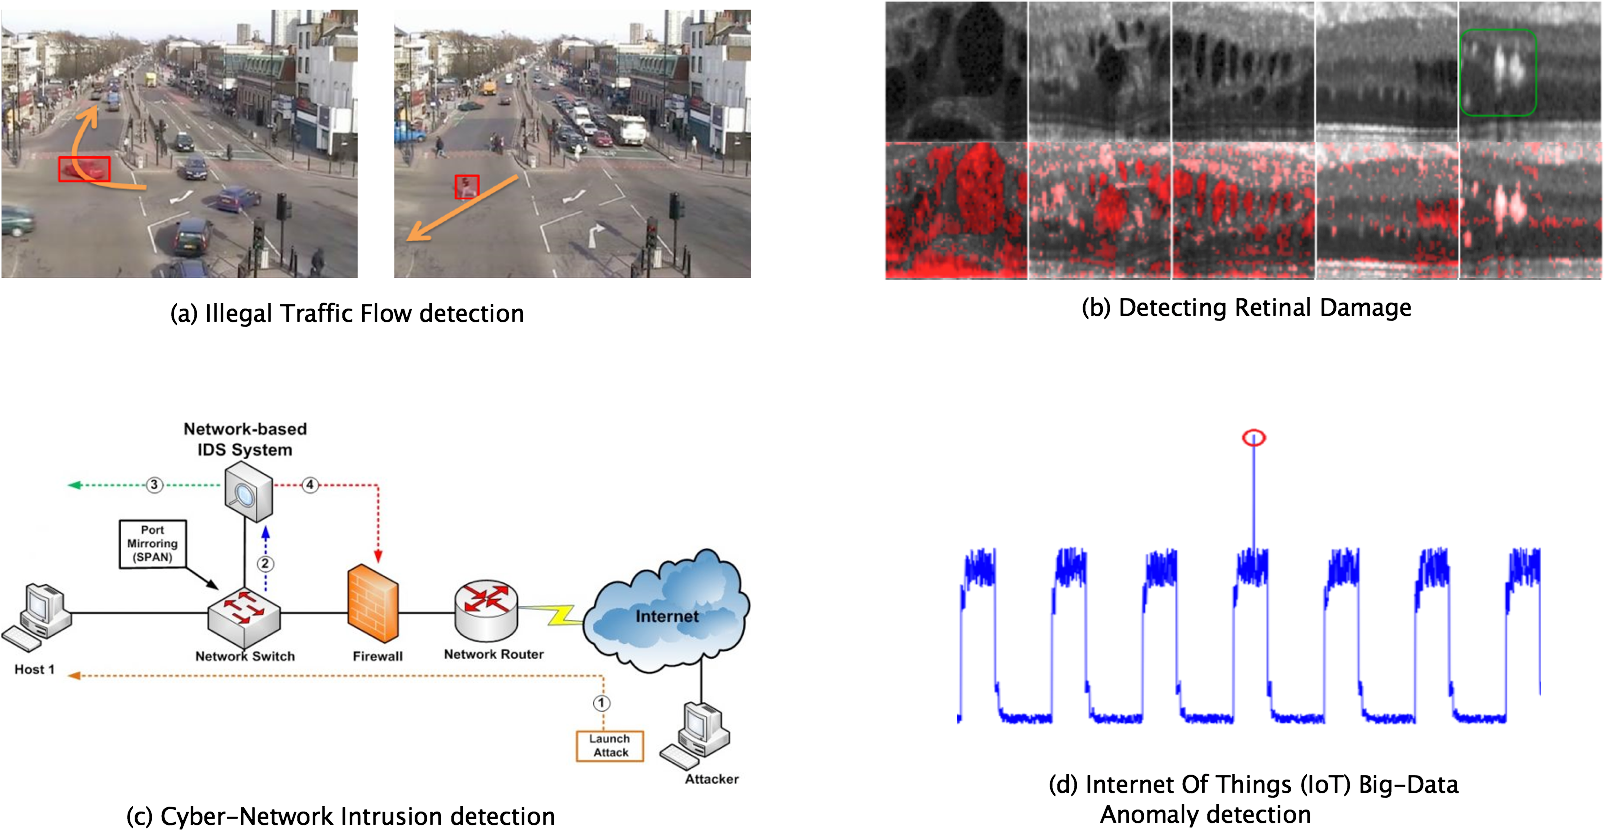
\includegraphics[scale=0.5]{images/applications}
\captionsetup{justification=centering}
\caption{Deep learning-based anomaly detection algorithms successfull applications.\\
(a) Video Survelliance, Image Analysis: Illegal Traffic detection~\cite{xie2017real}  ,  (b) Healthcare: Detecting Retinal Damage~\cite{schlegl2017unsupervised}\\
(c) Networks: Cyber-intrusion detection~\cite{javaid2016deep}  (d) Sensor Networks: Internet of Things (IoT) big-data anomaly detection~\cite{mohammadi2017deep} }
\label{fig:applications}
\end{figure}

The aim of this survey is two fold, firstly we present a structured and comprehensive overview of research methods in deep learning-based anomaly detection. Furthermore, we review the adoption of these deep-learning based methods for anomaly across various application domains and asess their effectiveness.

%anomalies
\section{ What are anomalies ?}
Anomalies  are also referred to as abnormalities, discordants, deviants, or outliers in the data mining and statistics literature~\cite{aggarwal2013introduction}.
% Anomaly Detection Definition
% \begin{figure}[h]
% 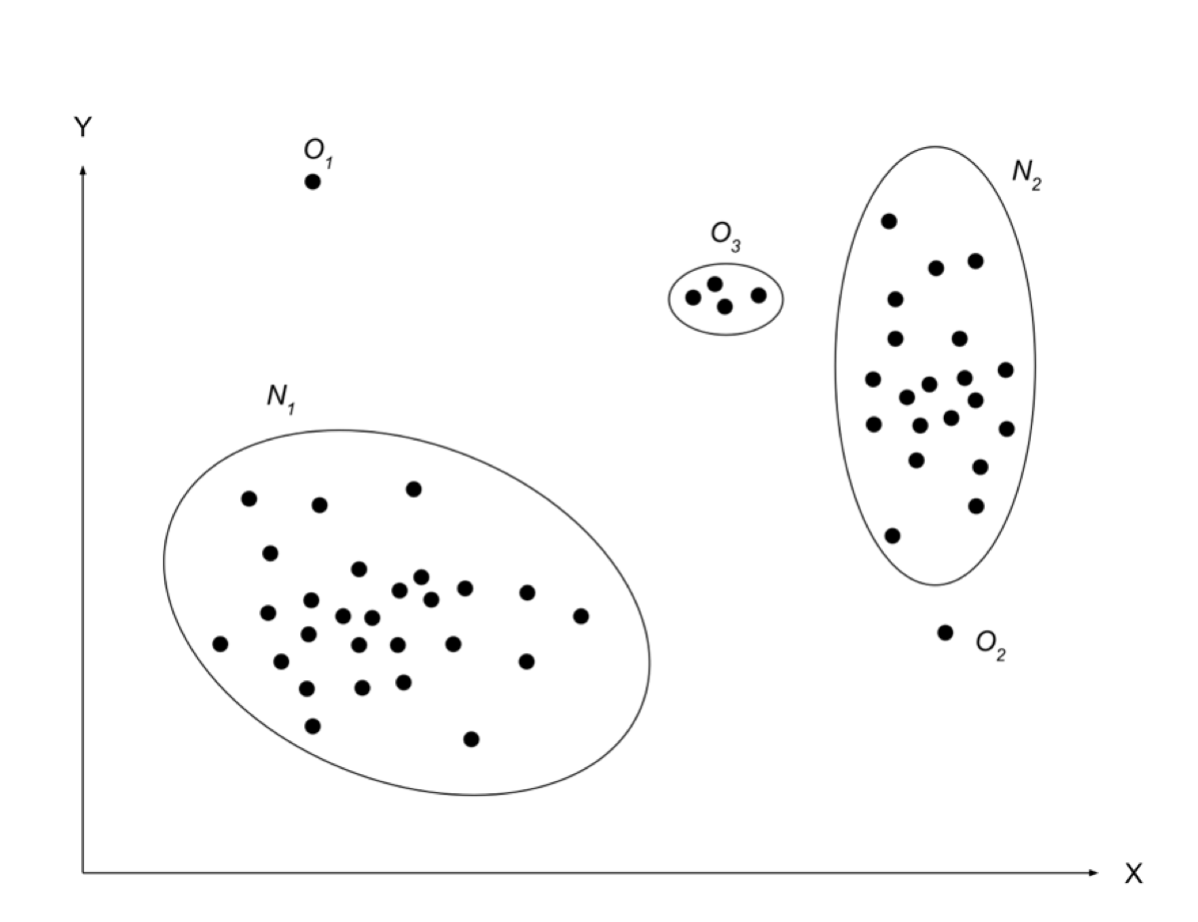
\includegraphics[scale=0.3]{images/anomalies.png}
% \caption{An illustration of anomalies in two-dimensional data set.}
% \label{fig:anomalies}
% \end{figure}

As illustrated in Figure ~\ref{fig:anomalies}, $N_{1}$ and $N_{2}$ are regions consisting of majority of observations and hence considered as normal data instance regions, whereas the region $O_{3}$, and data points  $O_{1}$ and $O_{2}$  are few data points which are located further away from the bulk of data points and hence are considered anomalies. Anomalies may arise due to several reasons, such as malicious actions, system failures, intentional fraud, etc. These anomalies reveal interesting insights about the data and are often convey valuable information about data. Therefore, anomaly detection considered an essential step in various decision-making systems.
% Novelty Detection Definition
% \begin{figure}[h]
% 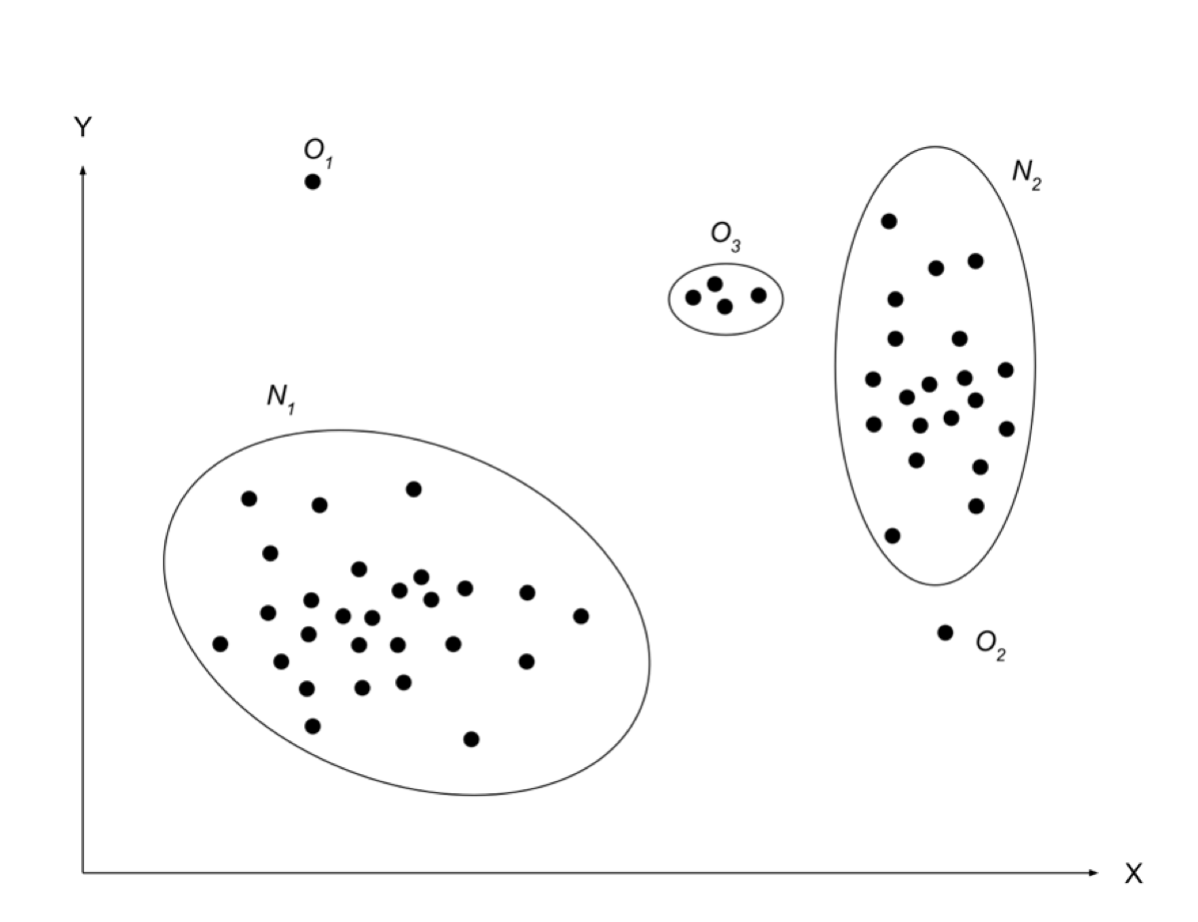
\includegraphics[scale=0.3]{images/anomalies.png}
% \caption{An illustration of anomalies in two-dimensional data set.}
% \label{fig:novelties}
% \end{figure}

% Begin of figure
\begin{figure}
  \centering
  \begin{minipage}{.48\linewidth}
    \centering
    % \subcaptionbox{}
      {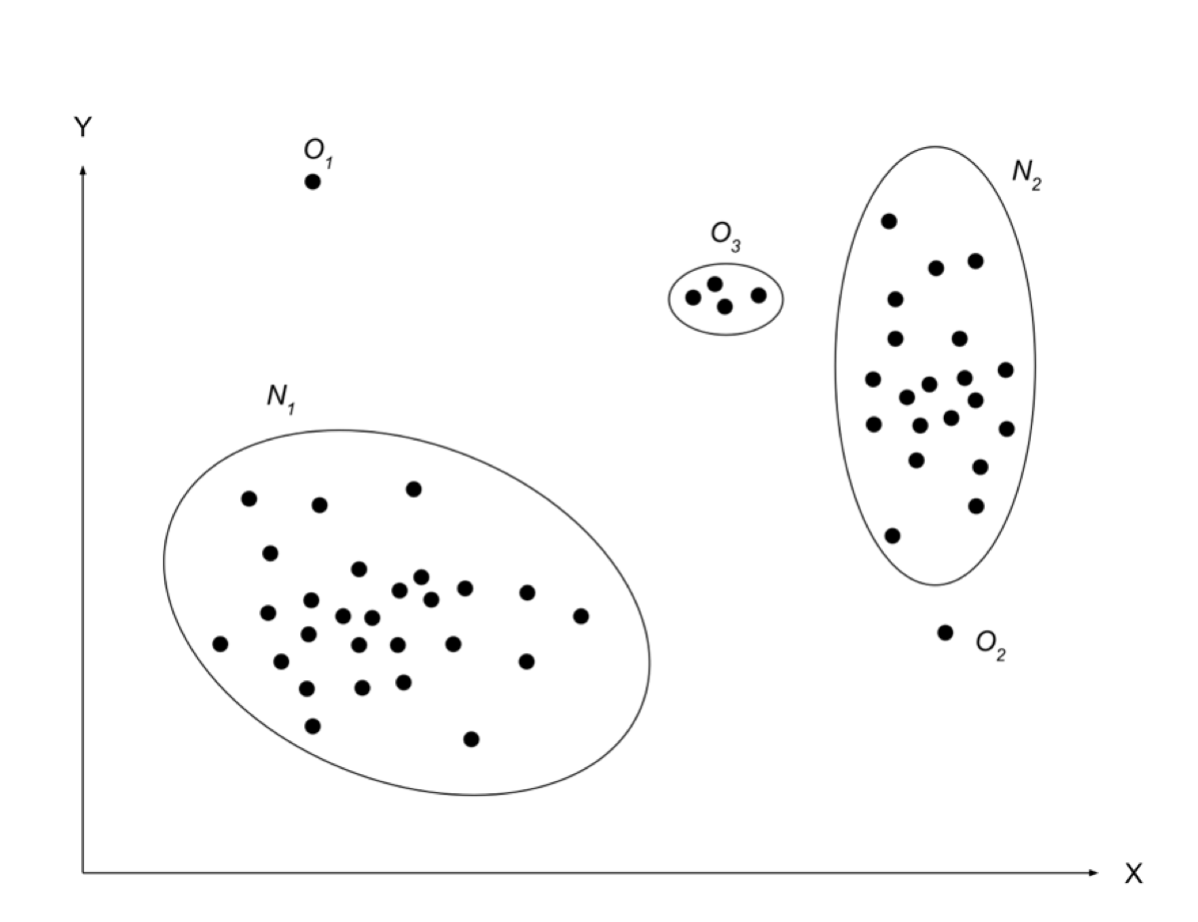
\includegraphics[scale=0.35]{images/anomalies.png}}
    \caption{Illustration of anomalies in two-dimensional data set.}
    \label{fig:anomalies}
  \end{minipage}\quad
  \begin{minipage}{.48\linewidth}
    \centering
    % \subcaptionbox{t}
      {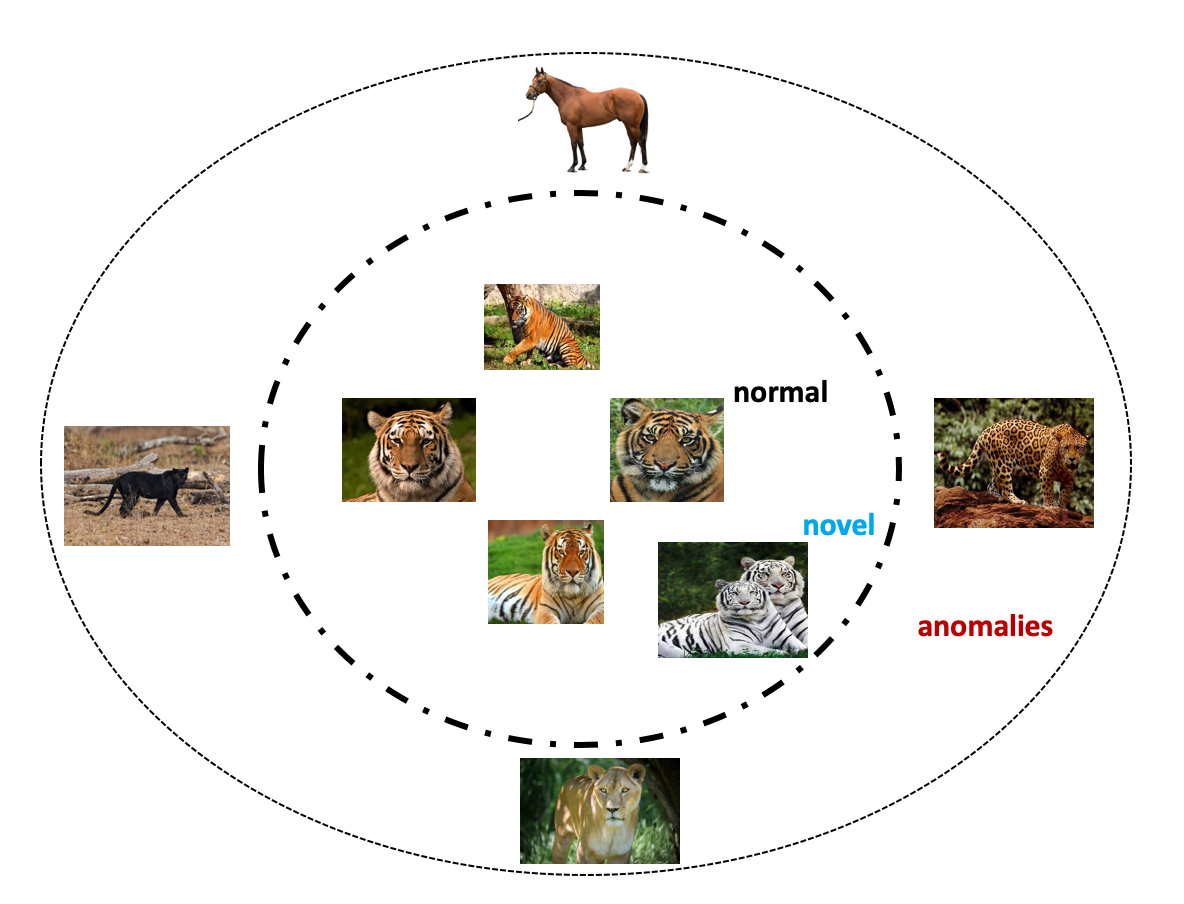
\includegraphics[scale=0.35]{images/novel.png}}
    \caption{Illustration of novelty in image data set.}
    \label{fig:novelties}
  \end{minipage}
  \bigskip

\end{figure}
% end of figure


% novelties
\section{What are novelties ?}
Novelty detection is the identification of novel (new) or unobserved patterns in the data.~\cite{miljkovic2010review}. The novelties detected are not considered as anomalous data points; instead they are incorporated into the normal data model. A novelty score may be assigned for these previously unseen data points, using a decision threshold score. ~\cite{pimentel2014review}.  The points which significanlty deviate from this decision threshold may be deemed as anomalies or outliers. For instance in Figure ~\ref{fig:novelties}  the images of \textit{(white tigers)} among normal tigers may be considered as novelty, while image of \textit{(horse, panther,lion and cheetah)} are considered as anomalies.
The techniques used for anomaly detection are often used for novelty detection and vice versa.



% Challenges : Motivation and challenges Why deep learning-based anomaly detection.
\section{Motivation and Challenges: Deep anomaly detection (DAD) techniques}
\begin{itemize}
\item Performance of traditional algorithms in detecting outliers is sub-optimal on complex image (e.g. medical images) and sequence data sets.
\item  Need for Large-scale anomaly detection : As the volume of data increases let's say to gigabytes then, it becomes nearly impossible for the traditional methods to scale to such large scale data to find outliers.
\item  Deep anomaly detection (DAD) techniques learn hierarchical discriminative features from data. This automatic feature learning capability eliminates the need of developing manual features by domain experts, therefore advocates to solve the problem end-to-end taking raw input data in domains such as text and speech recognition.
\item The boundary between normal and anomalous (erroneous) behavior is often not precisely defined  in several data domains and is constantly evolving. This lack of well defined representative normal boundary poses challenges for both conventional and deep learning-based algorithms.
\end{itemize}
% end itemize

% Begin Table
\begin{table} [ht!]
\centering
\captionsetup{justification=centering}
\caption{Comparison of our Survey to Other Related Survey Articles. \\1 \textemdash Our Survey,
2 \textemdash Kwon and Donghwoon ~\cite{kwon2017survey}, 5 \textemdash John and Derek ~\cite{ball2017comprehensive}\\
3 \textemdash Kiran  and Thomas ~\cite{kiran2018overview},            6 \textemdash Mohammadi and Al-Fuqaha ~\cite{mohammadi2017deep}\\
4 \textemdash Adewumi and Andronicus ~\cite{adewumi2017survey}       7 \textemdash Geert and  Kooi et.al ~\cite{litjens2017survey}.
}
\scalebox{0.8}{
\begin{tabular}{ |c|c|c|c|c|c|c|c|c|c| }
\hline
 & & 1&2&3&4&5&6&7 \\
\hline
\multirow{4}{6em}{Methods  }
&Supervised &\checkmark  & & & & & & \\
&Unsupervised &\checkmark & & & & & &  \\
&Hybrid Models & \checkmark& & & & & &  \\
&one-Class Neural Networks &\checkmark & & & & & &  \\
\hline
\multirow{8}{8em}{Applications  }
&Fraud Detection&\checkmark  & & &\checkmark & & & \\
&Cyber-Intrusion Detection&\checkmark  &\checkmark & & & & & \\
&Medical Anomaly Detection&\checkmark  & & & & & &\checkmark \\
&Sensor Networks Anomaly Detection&\checkmark  & & & &\checkmark & & \\
&Internet Of Things (IoT)
 Big-data Anomaly Detection&\checkmark  & & & & & \checkmark& \\
&Log-Anomaly Detection&\checkmark  & & & & & & \\
&Video Surveillance&\checkmark & &\checkmark  & & & & \\
&Industrial Damage Detection&\checkmark & & & & & & \\
\hline
\end{tabular}}
\end{table}
% End of Table


% Related Work
\section{Related Work}
Despite the substantial advances made by deep learning methods in many machine learning problems, there
is a relative scarcity of deep learning approaches for anomaly detection. Adewumi et.al~\cite{adewumi2017survey} provide a comprehensive survey of deep learning-based methods for fraud detection. A broad review of deep anomaly detection (DAD) techniques for cyber-intrusion detection is presented by Kwon et.al~\cite{kwon2017survey}. An extensive review of using DAD techniques in medical domain has been presented by Litjens et.al ~\cite{litjens2017survey}. An  overview of DAD techniques for Internet of Things (IoT) and  big-data anomaly detection is introduced by  Mohammadi et.al~\cite{mohammadi2017deep}. Sensor networks anomaly detection has been reviewed  by  Ball et.al~\cite{ball2017comprehensive}. The state-of-the-art deep learning based methods for video anomaly detection along with various categories has been presented in~\cite{kiran2018overview}. Although there are a number of reviews in applying DAD technqiues, there is shortage of comparative analysis of deep learning architecture adopted for outlier detection. For instance a substantial amount of research on anomaly detection is conducted using deep autoencoders, but there is lack of comprehensive survey of various deep architecture's best suited for a given data-set and application domain. We hope that this survey bridges this gap and provides a comprehensive reference for researchers and engineers aspiring to leverage deep learning for anomaly detection. Table I shows the set of research methods and application domains covered by our survey.

% The classification taxonomy is also present in this paper $https://www.ncbi.nlm.nih.gov/pmc/articles/PMC4836738/$
% This paper~\cite{erfani2016high} presents a hybrid approach of combining deep learning models in combination with other traditional techniques to identify outliers and obtained promising results.

% Anomaly Detection Taxonomy
\begin{figure}[h]
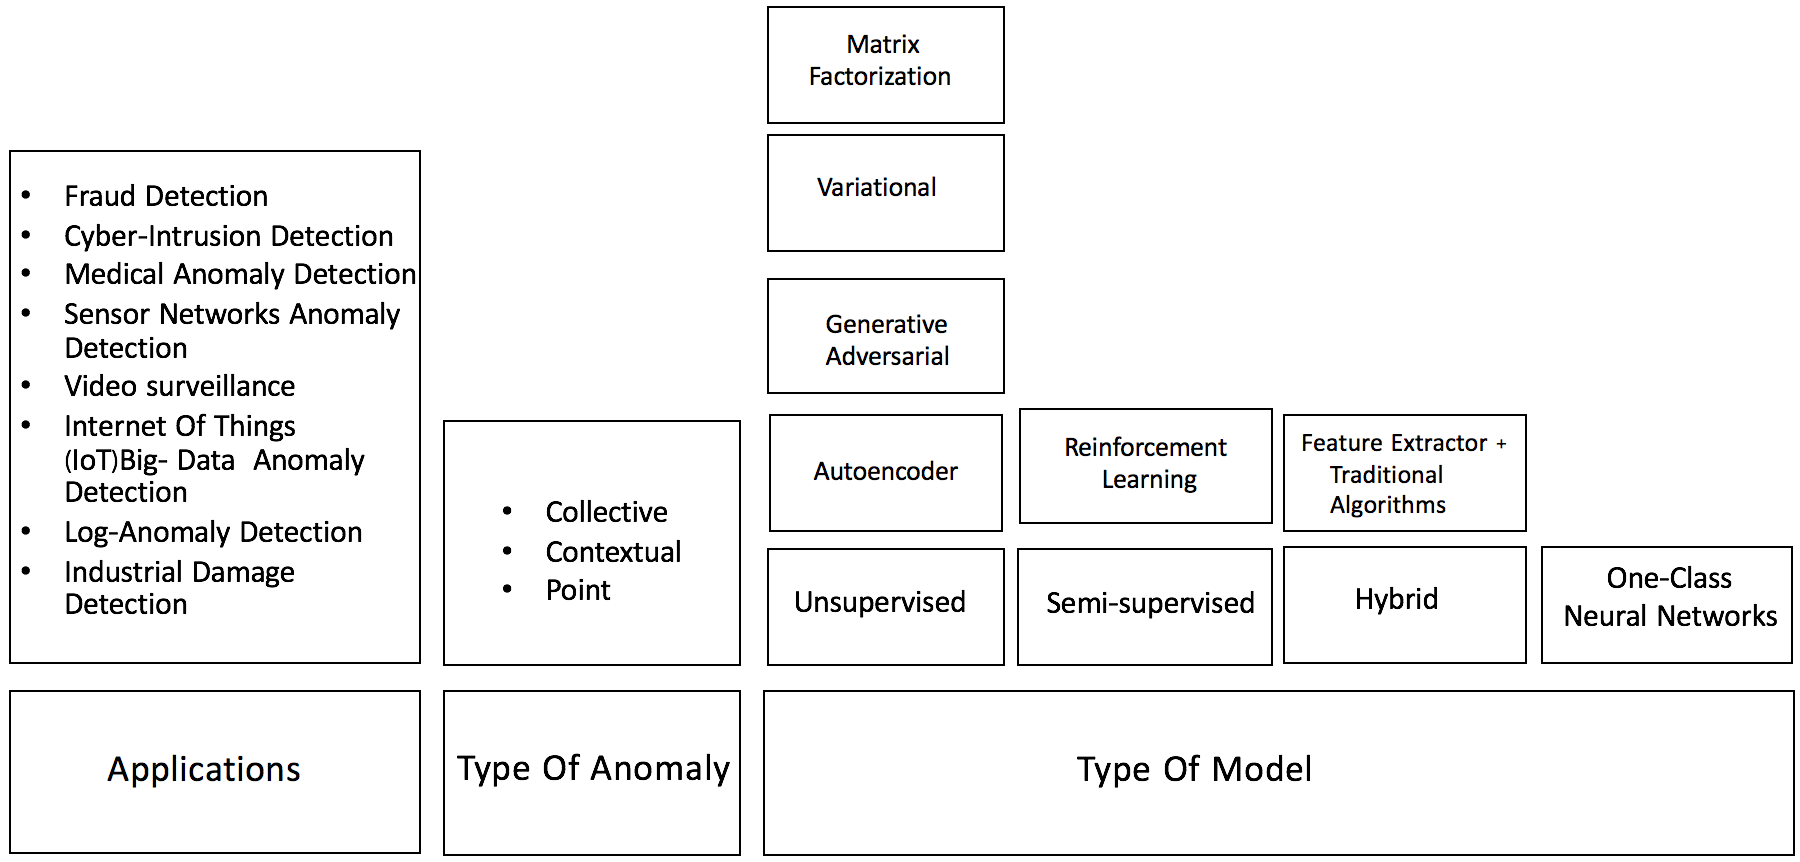
\includegraphics[scale=0.5]{images/AnomalyDetectionTaxonomy}
\caption{Key components associated with deep learning-based anomaly detection technique.}
\label{fig:surveyTaxonomy}
\end{figure}
% end of related work

%% Our Contributions
\section{ Our Contributions}
We follow survey approach of V.Chandola and A.Banerjee et.al~\cite{chandola2007outlier} for deep  anomaly detection (DAD). Our survey presents a detailed and structured overview of research and applications of DAD techniques. We summarize our main contributions as follows:
\begin{itemize}
\item Most of the existing surveys on DAD techniques either focus on a particular
application domain or specific research area of interest~\cite{kiran2018overview,mohammadi2017deep,litjens2017survey,kwon2017survey,adewumi2017survey,ball2017comprehensive}.
This review aims to provide a comprehensive outline of state-of-the art research in DAD techniques as well as several real world applications these techniques are discussed.
\item In recent years a number of new deep learning based anomaly detection techniques  with greatly reduced computational requirements have been developed. The purpose of this paper is to survey these techniques and classify them into organised schema for better understanding. We introduce two more sub-categories Hybrid models ~\cite{erfani2016high} and one-class neural networks techniques~\cite{chalapathy2018anomaly} as illustrated in Figure~\ref{fig:surveyTaxonomy} based on the choice of training objective. For each categories we discuss both the assumptions and techniques adopted for best performance. Furthermore within each category, we also present the challenges, advantages and disadvantages and provide an overview of computational complexity of DAD methods.
\end{itemize}

% Organization of the paper
\section{Organization}
This survey is organized by following structure described in Figure~\ref{fig:surveyTaxonomy}.
In Section~\ref{sec:aspectsOfAnomalyDetection}, we identify the various aspects that determine the formulation of the problem and highlight the richness and complexity associated with anomaly detection.
We introduce and define two types of models: contextual and collective or group anomalies. In Section~\ref{sec:applicationsOfDLAD}, we briefly describe the different application domains to which deep learning-based anomaly detection has been applied. In subsequent sections we provide a categorization of deep learning-based techniques based on the research area to which they belong.  Based on training objectives employed and availability of labels  deep learning-based anomaly detection techniques  can be categorized into supervised (Section~\ref{sec:supervisedDAD}), unsupervised (Section ~\ref{sec:unsupervisedDAD}), hybrid (Section~\ref{sec:hybridModels}), and one-class neural network  (Section~\ref{sec:oneclassNN}). For each category of techniques we also discuss their computational complexity for training and testing phases. In Section~\ref{sec:typeBasedAD} we discuss  point, contextual, and collective (group) deep learning-based anomaly detection techniques. We present some discussion of the limitations and relative performance of various existing techniques in Section~\ref{sec:relativeSOW}. Section~\ref{sec:conclusion} contains
concluding remarks.




% Group deviation detection involves the discovery of group behaviours which significantly deviate from  expected   patterns. With  increased availability of multifaceted information, there is a growing trend towards research involving groups or collections of observations.   Group anomaly detection (GAD) is the process of identifying groups that are not consistent with regular group behaviours while group change detection (GCD) estimates significant deviations in the state of a group over  time. Since both GAD and GCD problems share fundamental ideas, this  Even though GAD usually involves time-independent applications and GCD relates to time-dependent groups, both problems share a common framework  and  fundamental ideas.
% thesis elaborates on group deviation detection techniques in static and dynamic situations.


% % \subsection{Definition of Groups} %
% A group is simply defined as a collection of two or more related data instances.    %F\~{a}rber et al. \cite{ClusterEval} even discusses how known group labels may not correspond to inherently clustered points.
% In GAD, a group anomaly has  significantly different  statistical properties  with respect to other groups whereas GCD involves detecting  a significant change in a group  with respect to past behaviour.   Group structures may be known a priori such as words in a document otherwise when group   memberships between instances are unknown, additional information or clustering algorithms are required.
% %  Thus the initial definition of groups greatly  affects subsequent analysis and results of detecting group deviations.




% More specifically,  Xiong et al.  \cite{MGM} categorise group deviations as either point-based or distribution-based for GAD applications.   Point-based anomalous groups are where all of the members are also pointwise anomalies. Similarly in GCD, a point-based group change signifies that a large proportion of  time series in a group exhibit significant deviations.   On the other hand, a  distribution-based group anomaly is where  individual  instances conform to regular patterns however the collection of points is anomalous. Likewise, a distribution-based change in a group over time occurs when individual time series exhibit regular behaviour however the  collective process is significantly different to historical patterns.



% \begin{figure}[h]
% \centering
% % \begin{subfigure}[b]{0.6\textwidth}
% %                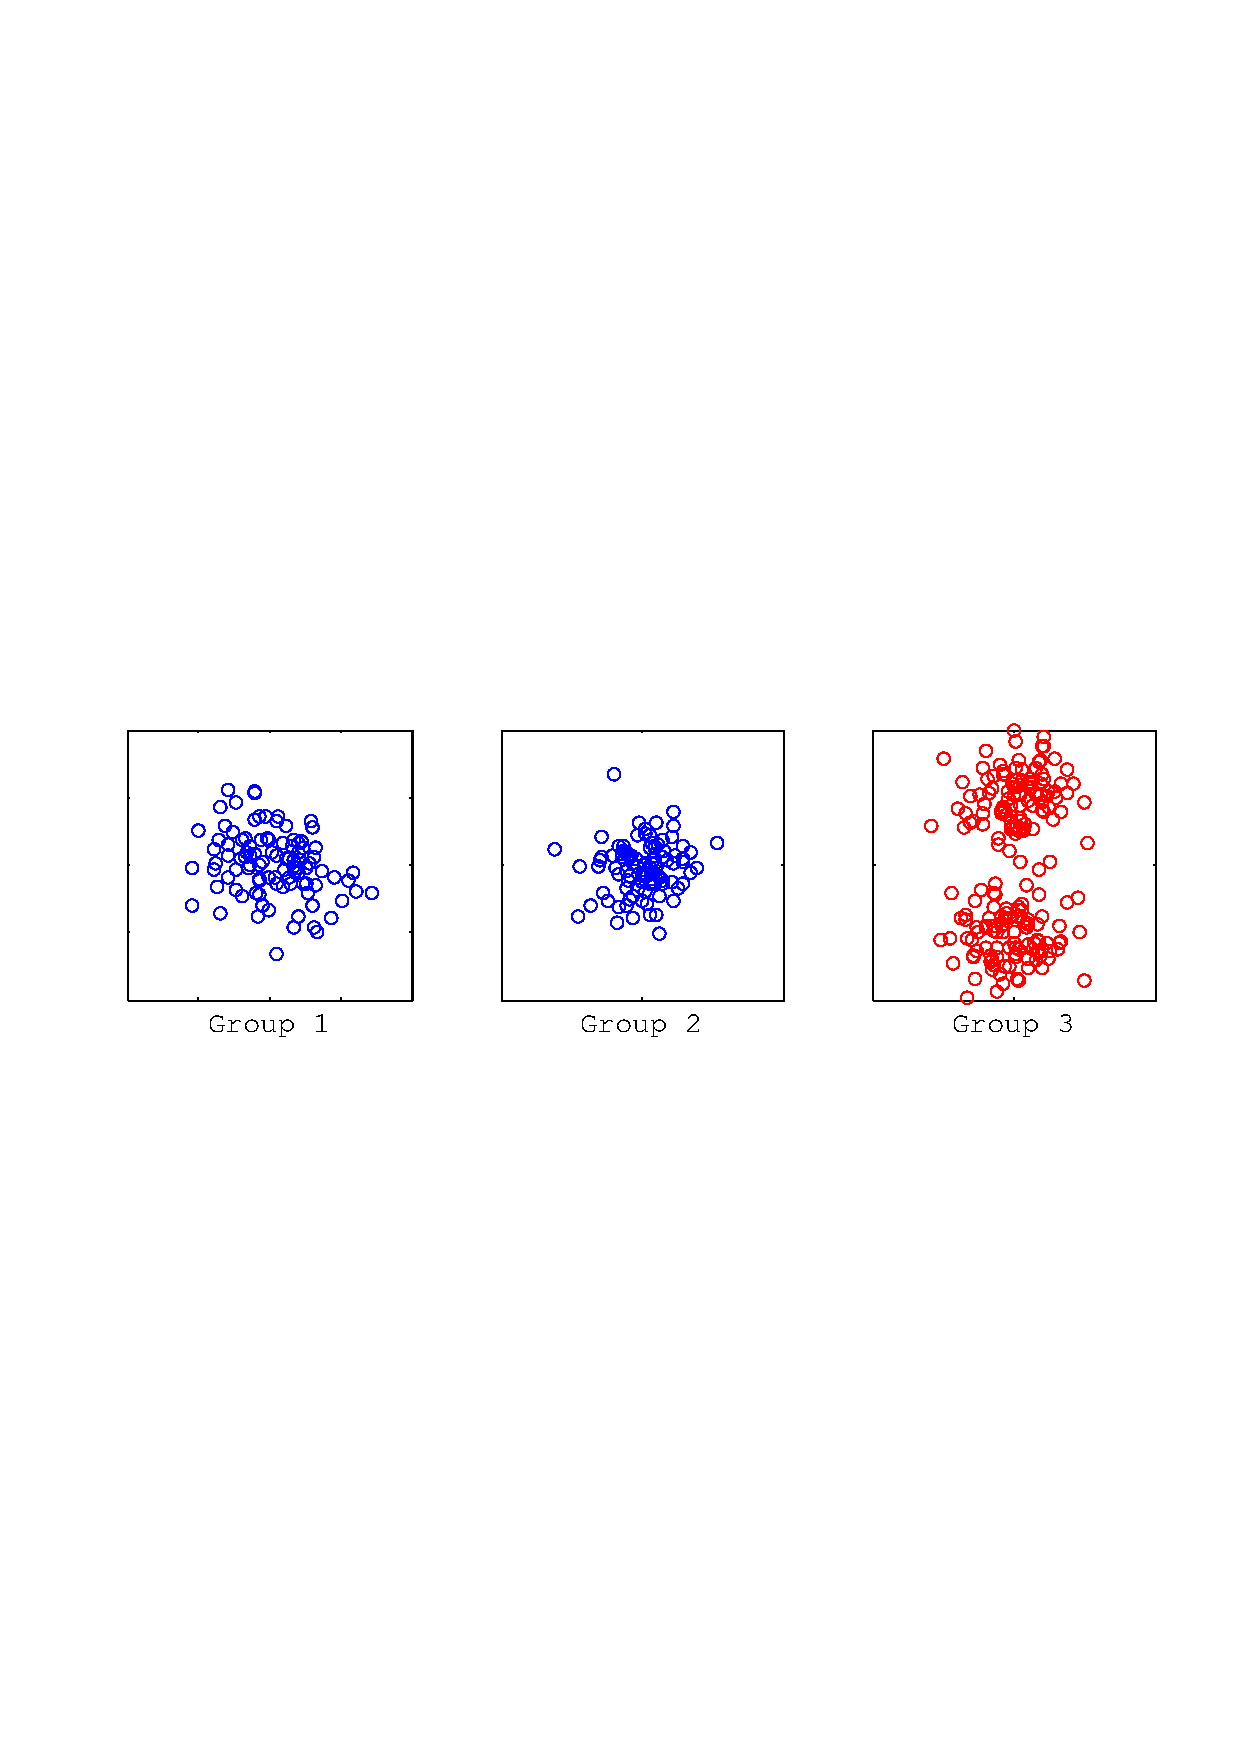
\includegraphics[width=\linewidth,trim=3cm 12cm 3cm 12cm]{FIGURES/Ex1}
% %                \caption{A significant deviation in scale or shape.}
% %        \end{subfigure}%
%  \begin{subfigure}[b]{1\textwidth}
%                 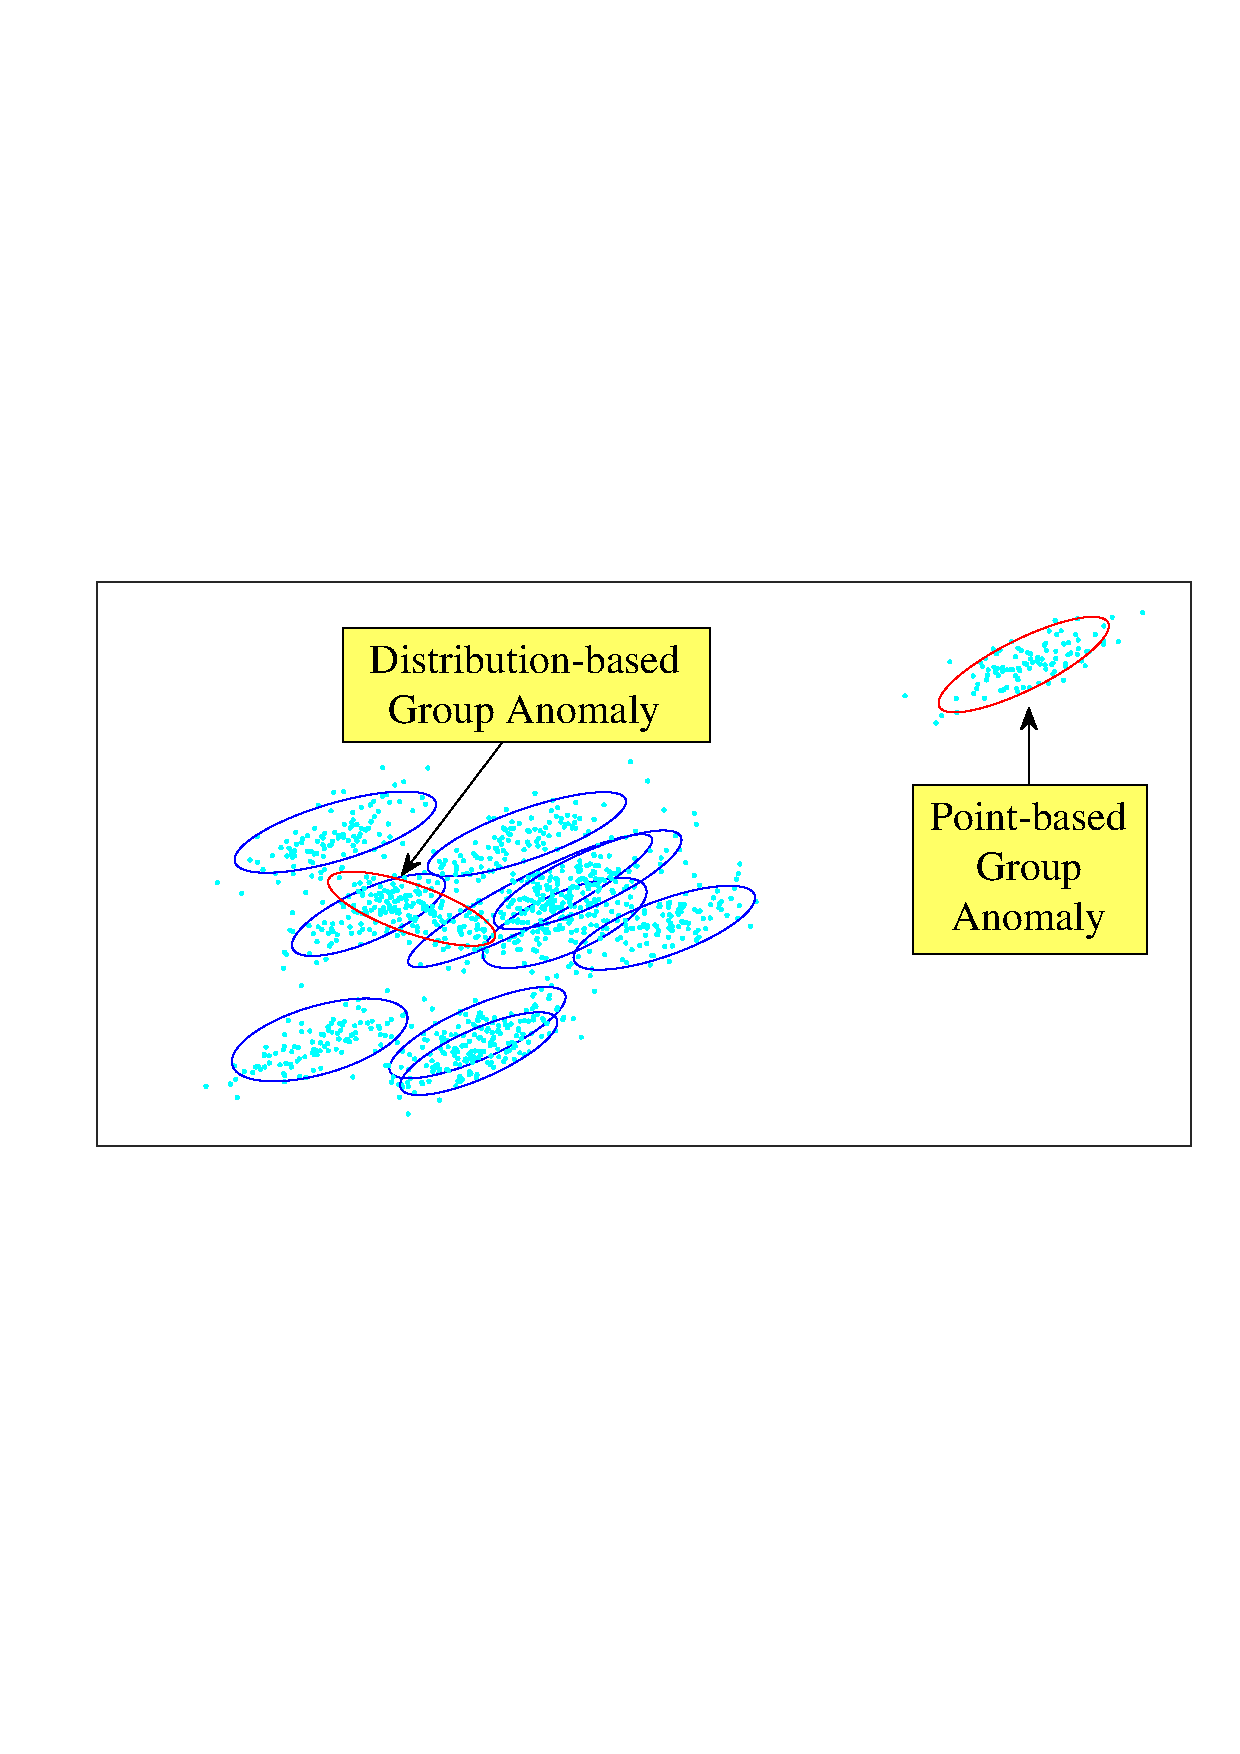
\includegraphics[width=9cm,
%                 height=5cm,trim=0cm 10cm 6cm 10cm]{FIGURES/gad_ex}
%                 \caption{Two types of group anomalies; point-based group anomaly is a collection of anomalous points  %that are anomalous with respect to a central location
%                  whereas in this example, a  distribution-based group anomaly contains non-anomalous observations however as a  collection,  significantly differs with a rotated  correlation structure.                    }
%         \end{subfigure}%
% \hfill
% \vspace{2mm}
% \vfill
%  \begin{subfigure}[b]{1\textwidth}
%  \centering
%                 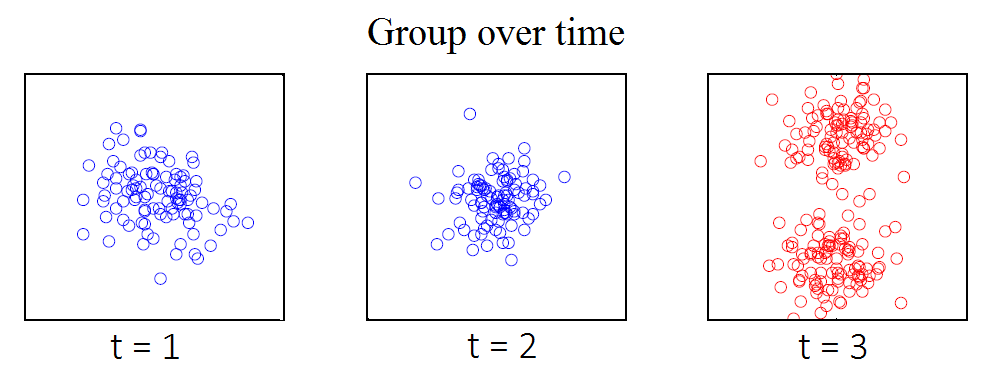
\includegraphics[width=10cm, height=4cm,trim=0cm 0cm 0cm 0cm]{FIGURES/gcd_ex}
%                 \caption{ Distribution-based group change at $t=3$ has significantly different  scale and shape.
% }
%   \end{subfigure}%
% \caption{Examples of group behaviours that clearly deviate in terms of different statistical properties.
% }
% \label{Fig:Intro1}
% \end{figure}

%  Figure \ref{Fig:Intro1}  highlights examples of group deviations that occur in  GAD and  GCD applications. For GAD, a point-based group anomaly  differs by central location whereas the distribution-based group anomaly has a rotated correlation structure. The GCD example illustrates   a group change as a significant deviation in scale and shape over time.  In real-world applications, Xiong et al. \cite{MGM} detect  rotated galaxy clusters whereas Chen et al. \cite{GLETS}  identify deviating scale and shape of a  stock portfolio over time.


% GAD and GCD methods have many advantages over  pointwise methods for detecting group deviations.
% %Pointwise anomaly and change detection focus on the study of individual data instances that do not conform with the expected pattern.
%  Many pointwise anomaly detection methods are also not compatible  in detecting  group deviations so  more specialised techniques are required.
%  For example,  Muandet et al.	\cite{OCSMM} detect Higgs bosons as a group of collision events  in high energy particle physics while a group of multiple sensor networks in Chen and Yu \cite{chen2016collaborative}, allow for a robust  detection of  distributed denial-of-service attacks. Group deviation detection  techniques also result in fewer false positives than pointwise approaches as a greater number of observations occur in real-world group applications. %provide a better characterization of group behaviours.



% Detecting group anomalies has a variety of interesting real-world results. % physical real-world  applications.  %that motivate different avenues of research.
%   Muandet et al.	\cite{OCSMM} investigate GAD in high energy particle physics where Higgs bosons are observed as slight excesses in a collection of collision events rather than individual  instances. In Guevara et al. \cite{SMDD}, an anomalous galaxy cluster is identified by an irregular proportion of color pixels while Xiong et al. \cite{FGM}  analyse unusual vorticity in fluid turbulence data.
% %where a group anomaly represents  in  fluid dynamics.
% Textual data is also studied for GAD where a document is considered a group of words.
% Using word inputs from scientific publications, Yu et al. \cite{GLAD}  %investigate  in order to understand the structure of certain research communities. I
% detect  possible irregular communities of co-authors that reveal unusual research trends.  By analysing documents from news articles, Soleimani and Miller \cite{ATD} discover novel topics in a document corpus.   Using text data from Amazon reviews, Mukherjee et al.  \cite{GroupReviewSpam} examine groups of spammers that collaborate in writing fake reviews.

%  %infer regular topics   such as $`\mathtt{rec.sport.baseball}'$  and $`\mathtt{ talk.politics.misc}'$. An anomalous cluster in this case consists of novel topics that are unobserved in the training corpus such as $`\mathtt{rec.sport.hockey}'$ and \\$`\mathtt{talk.politics.mideast}'$.

% %There are many other applications where GAD and GCD techniques offer interesting results.

%   A group over time for GCD is also studied across a variety of domains.  Wong et al. \cite{wong-rule} %investigate different demographic groups admitted to  emergency departments in hospitals in a major US city.   A
%    detect significant changes in demographic groups that are admitted to  emergency departments where changes represent  potential disease outbreaks.
%   Chen et al. \cite{GLETS} monitor how a group of  stocks
%   may disband with dissimilar behaviors over time while seemingly uncorrelated time series may form a more cohesive collection.   Using multiple sensor data, Xie and Siegmund  \cite{xie2013} explore sequential change detection in a proportion of time series in a group over time.
%   Another example of real-world GCD event occurred when  five of the largest private health insurers in Chile colluded to unfairly reduced  coverage of healthcare plans over time \cite{Chile}.   Thus there are many interesting and meaningful insights that are gained from GAD and GCD applications.
% The  main contributions  of our thesis are  summarised as follows: %\vspace{-1mm}
% \begin{enumerate}
% %\item {\bf Clearer Understanding:}
% %This survey provides an underlying structure for   both group anomaly detection (GAD) and group change detection (GCD) problems.      % Figure \ref{Fig:Framework}  builds upon the anomaly detection from Chandola \cite{Chandola}
% \item {\bf Detailed Overview:}
%  We clearly formulate the problem of group anomaly detection (GAD) and group change detection (GCD) with detailed descriptions of state-of-the-art techniques. %Although deep generative models have been applied in various image applications, they have not been applied to the GAD problem. % of detecting group anomalies.
% \item {\bf Static GAD}: Deep generative models (DGMs) are proposed for solving the GAD problem for complex group distributions with a high detection performance under certain conditions.
% \item {\bf Dynamic GCD:} We propose the GT$\Delta$ algorithm  for sequentially detecting temporal changes in  a group of stochastic processes with advantages such as a robustness to outliers,  better interpretation and effective detection results.
% \end{enumerate}
